\documentclass{beamer}

\usepackage[utf8]{inputenc}

\usepackage{utopia} %font utopia imported

\usetheme{Copenhagen}
\usecolortheme{beaver}

%Information to be included in the title page:
\title{Linux Workshop}
\author{Mitchell Dzurick}
% \institute{UofA}
\date{11/09/2022}

\AtBeginSection[]
{
  \begin{frame}
    \frametitle{Table of Contents}
    \tableofcontents[currentsection]
  \end{frame}
}

\begin{document}

\frame{\titlepage}


\begin{frame}
\frametitle{What are we doing Today}
\tableofcontents
\end{frame}


\section{Introduction}

\frame{
	\frametitle{Presentation Source Code}
	This presentation and source code can be found at \\
	
	\url{https://github.com/mitchdz/IEEE_Linux_Workshop}
}

\frame{
	\frametitle{About Me}
	\begin{columns}
		\column{0.38\linewidth}
			\centering
			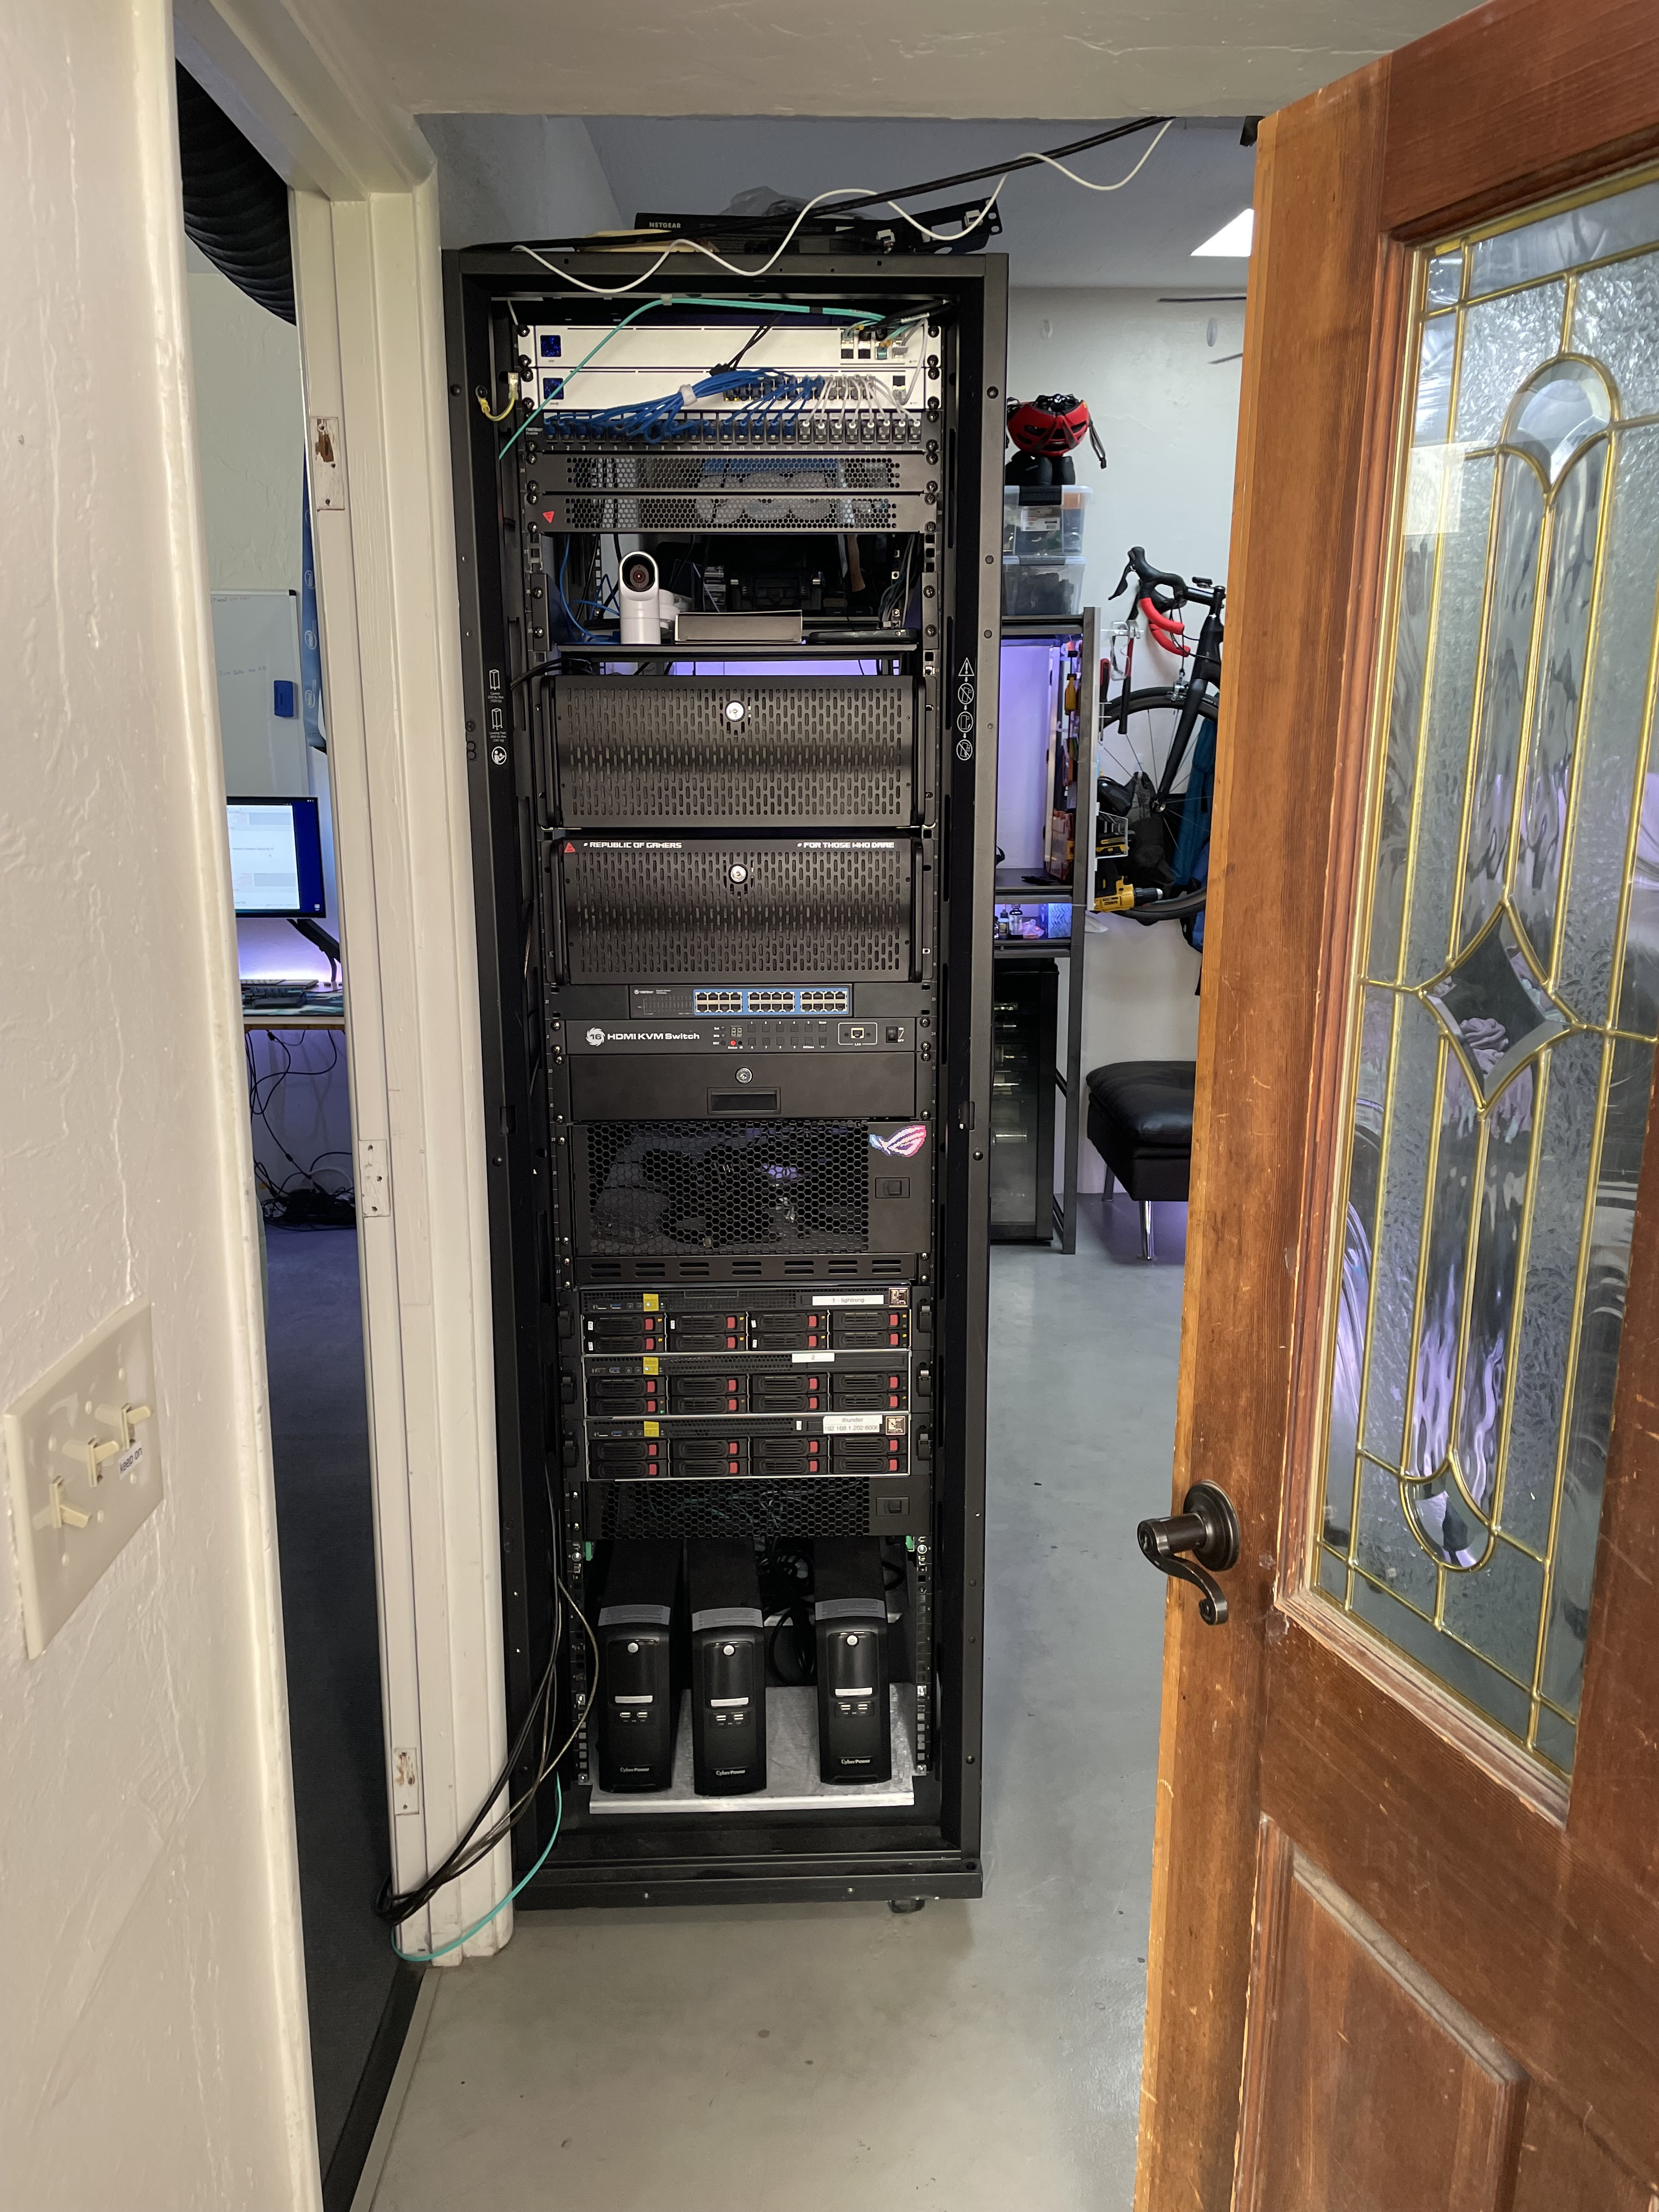
\includegraphics[width=\textwidth,height=\textheight,keepaspectratio]{images/my_server.jpg}
		\column{0.58\linewidth}
			\begin{itemize}
				\item UA Alum - Masters in Computer Engineering '21
				\item Really likes Linux
				\item Currently Systems Validation Engineer for Intel QAT Compression service
				\item Used to build Custom Linux images for Intel Trusted Edge Platform
			\end{itemize}
			$\leftarrow$ Has a large space heater
	\end{columns}
}

\frame{
	\frametitle{Motivation}
	\begin{itemize}
		\item Linux isn't taught well in school
		\begin{itemize}
			\item often employers expect you can use it
		\end{itemize}
		\item I love this stuff
		\item You might love this stuff too
	\end{itemize}
}

\frame{
	\frametitle{Foreword}
	Who is this workshop for?
	\begin{itemize}
		\item New and intermediate Linux users alike
	\end{itemize}
	What can you expect to learn today?
	\begin{itemize}
		\item Enough to understand what Linux is
		\item Basic Linux commandline operation
		\item Tips on system usage
	\end{itemize}
}

\section{Computer Boot Flow}

\frame{
	\frametitle{Boot Sequence}
	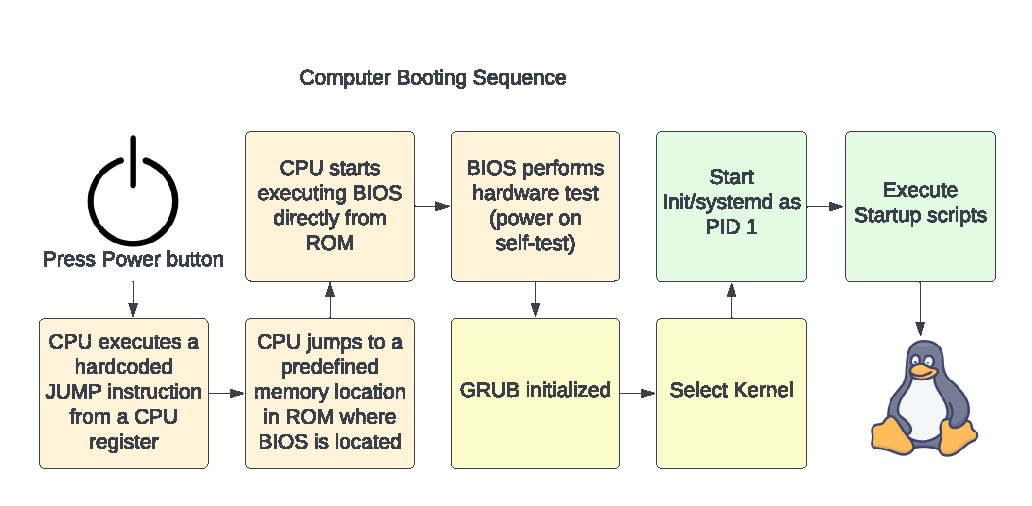
\includegraphics[width=\textwidth,height=\textheight,keepaspectratio]{images/Boot_Sequence.pdf}
}

\frame{
	\frametitle{Quick note on SysVInit/Systemd}
	SysVInit (init.d) and systemd are competing system and service managers. They are the most popular in Linux distros.
	
	\textbf{SysVInit} commands look like so:
	\begin{itemize}
		\item sudo /etc/init.d/apache2 status
		\item sudo service apache2 status
	\end{itemize}
	
	\textbf{systemd} commands look like so:
	\begin{itemize}
		\item sudo systemctl status apache2.service
	\end{itemize}
	
	Arch/Debian/Ubuntu/CentOS/Fedora/Manjaro/RHEL are some examples that use systemd by default \\
	Gentoo has SysV default
}

\frame{
	\frametitle{What is a system and service manager?}
	The system and service manager are two different jobs, but usually a single tool does both.
	\begin{itemize}
		\item System manager is an \textbf{init} system used to bootstrap user space
		\item Service manager is a tool to manage and interact with \textbf{daemons} and user processes
	\end{itemize}
	There are many alternatives to SysVInit and systemd, for example we have:\\
	MSConfig, OpenRC, s6, Launchd, eudev, runit, bootchart
}

\frame{
	\frametitle{Linux Systems Processes}
	There are 3 types of Processes you will find in a Linux System
	\begin{itemize}
		\item User Processes
		\item Daemon Processes
		\item Kernel Processes
	\end{itemize}
	\begin{center}
		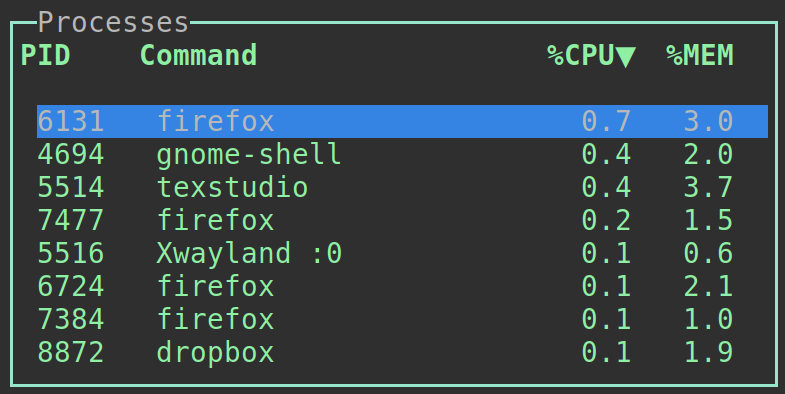
\includegraphics[width=0.6\textwidth,height=0.6\textheight,keepaspectratio]{images/processes.png}
	\end{center}
}

\frame{
	\frametitle{User Processes}
	\begin{itemize}
		\item Initiated by a regular user
		\item Runs in user space
		\item often interact with it visually
	\end{itemize}
	Below is an example of running a command in a user process, the common update command on Debian distributions is one system administrators will know well.
	
\includegraphics[width=\textwidth,height=\textheight,keepaspectratio]{images/apt_update.png}
}

\frame{
	\frametitle{Daemon Processes}
	\begin{itemize}
		\item Designed to be ran in the background
		\item No user interface
	\end{itemize}
	You can easily convert a user process into a daemon by simply appending \& to the end of the command
	
\includegraphics[width=\textwidth,height=\textheight,keepaspectratio]{images/apt_upgrade_daemon.png}
	
	NOTE: the daemon is attached to the shell in this case, so if you close the shell, the process will stop. You can prepend the utility 'nohup' before the command to alleviate that
}

\frame{
	\frametitle{Kernel Process}
	AKA kproc
	\begin{itemize}
		\item Only run in Kernel Space
		\item Very similar to Daemon Processes, except they can access Kernel Data Structures
		\item Just need to know that they are very powerful and we won't be creating our own today 
	\end{itemize}
	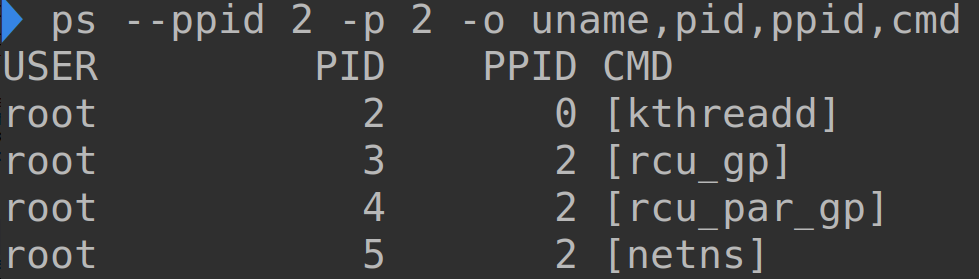
\includegraphics[width=\textwidth,height=\textheight,keepaspectratio]{images/list_kproc.png}
}


%%%%%%% INTRODUCTION TO LINUX
\section{Introduction to Linux}

\frame{
	\frametitle{What is Linux?}
	\begin{itemize}
		\item Linux is a Kernel
		\item All operating systems have a kernel
		\item The kernel is a piece of software that tells your userspace applications how to talk to the hardware
	\begin{center}
		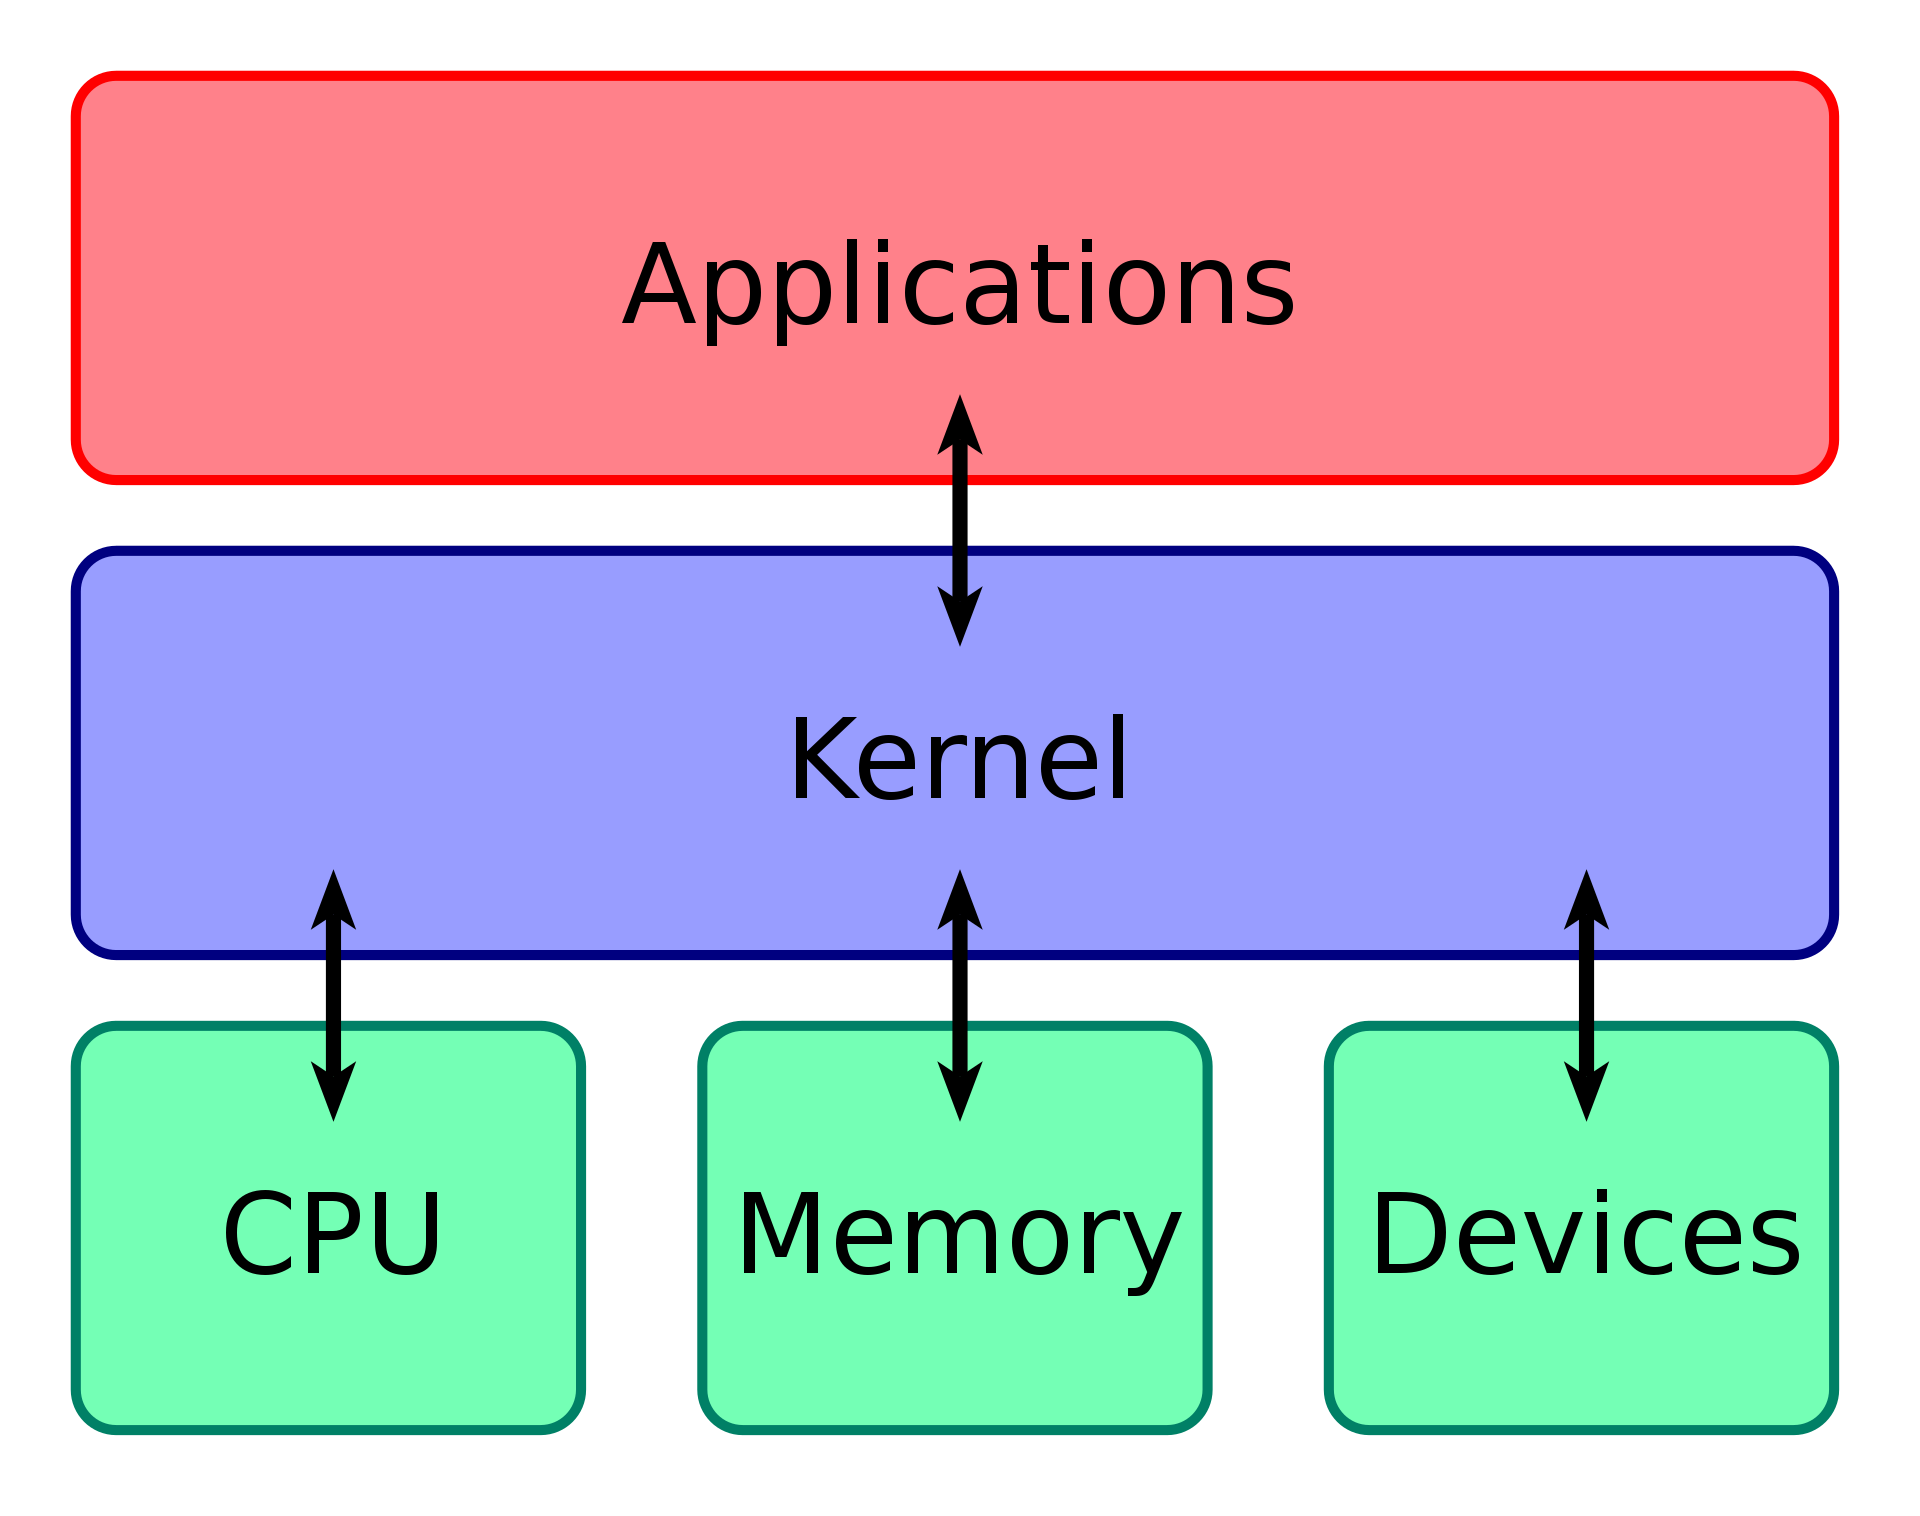
\includegraphics[width=0.5\textwidth,height=0.5\textheight,keepaspectratio]{images/1920px-Kernel_Layout.png}
	\end{center}
	\end{itemize}
}

\frame{
	\frametitle{Monolithic versus microkernel}
	\begin{center}
		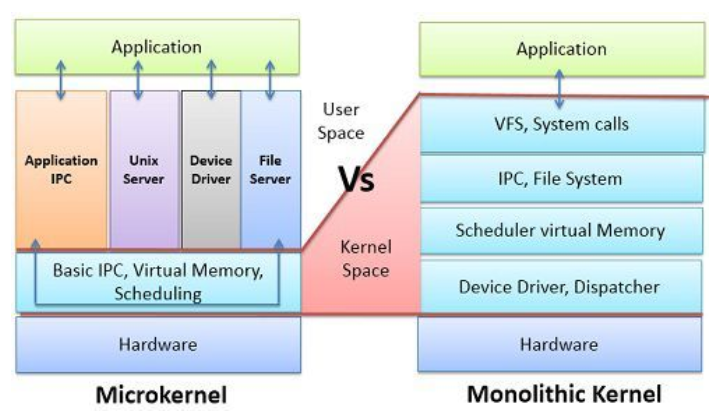
\includegraphics[width=\textwidth,height=\textheight,keepaspectratio]{images/mono_vs_microkernel.png}
	\end{center}
}


\frame{
	\frametitle{What is a Linux Distribution?}
	A Linux distribution is a \textbf{collection of software packages} that make up a full-fledged Operating System. Here's just a few:
	
	Ubuntu, Fedora, Arch, Kubuntu, Scientific Linux, Parrot OS, NixOS, Hannah Montana Linux, Puppy Linux
	
	\begin{center}
		
\includegraphics[width=\textwidth,height=\textheight,keepaspectratio]{images/puppy-linux-logo.jpeg}
	\end{center}
}

\frame{
	\frametitle{What is a Linux Distribution? - Package Manager}
	Package management is a very important part of choosing a linux distro, and each package  manger has it's own pros/cons
	
	\begin{itemize}
		\item \textbf{apt} - Debian based distros (ubuntu, kali linux, ect...) (deb based)
		\item \textbf{yum/dnf} - Fedora, CentOS, RHEL (rpm based)
		\item \textbf{pacman} - Arch
		\item \textbf{zypp} - OpenSUSE (rpm based)
	\end{itemize}
}

\frame{
	\frametitle{What is a Linux Distribution? - Linux Distribution Timeline}
	\url{https://upload.wikimedia.org/wikipedia/commons/1/1b/Linux_Distribution_Timeline.svg}
}

\frame{
	\frametitle{Introduction to Filesystems}
	The filesystem (often referred to as fs) is a very important part of Linux (and all operating systems)
	
	The fs is just a \textbf{method and data structure that the OS uses to control how data is stored and retrieved}. Common filesystems are ext2, ext3, ext4, btrfs, squashfs, FAT, NTFS
	
	\begin{center}
		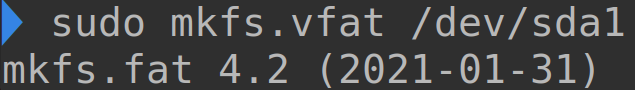
\includegraphics[width=\textwidth,height=0.9\textheight,keepaspectratio]{images/mkfs.vfat.png}
	\end{center}
}


\frame{
	\frametitle{Everything is a file}
	Just like the title says, everything is a file.
	\begin{itemize}
		\item Text document? file
		\item driver? file
		\item flash drive? file
		\item network attached storage? file
		\item hardware accelerator (TPM,QAT)? file
		\item 2D printer attached via USB cable? file
	\end{itemize}
}


\frame{
	\frametitle{Introduction to Filesystem Hierarchy Standard (FHS)}
	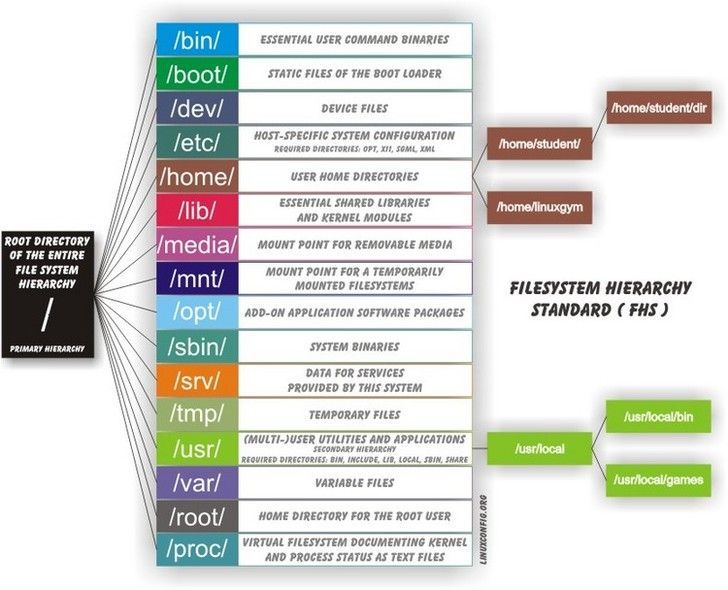
\includegraphics[width=\textwidth,height=0.9\textheight,keepaspectratio]{images/Directory-Filesystem-Hierarchy-Standard.jpg}
}


\frame{
	\frametitle{Linux Kernel vs. Userspace}
	The kernel is the core of the operating system and has full access to all memory and machine hardware, whereas userspace does not have that access
	
	\begin{center}
		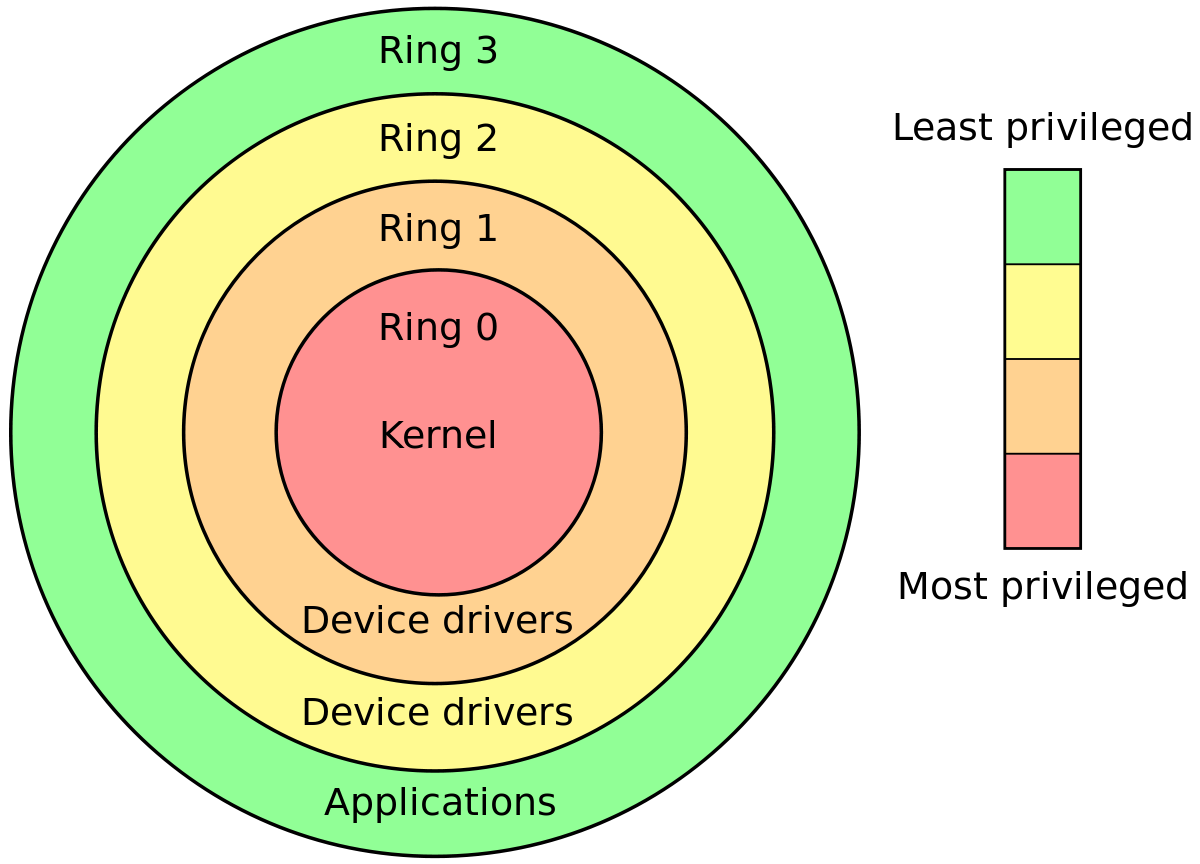
\includegraphics[width=0.5\textwidth,height=0.5\textheight,keepaspectratio]{images/kernel_rings.png}
	\end{center}
}

%%%%%%%%%%%%%%%% ALL ABOUT SHELLS

\section{All about Shells}

\frame{
	\frametitle{Well, what is a shell?}
	The shell is an user space program that takes commands from the keyboard and gives them to your operating system to perform
	
	\textbf{Commandline}\\
	The commandline has a prompt which is what you type commands into
	\begin{center}
		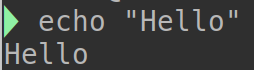
\includegraphics[width=0.5\textwidth,height=0.5\textheight,keepaspectratio]{images/echo_hello.png}
	\end{center}
	
}




\frame{
	\frametitle{Bourne Shell}
		\begin{itemize}
			\item The Bourne shell was the default shell in version 7 of unix, and was created in \textbf{1977}
			\item still present in most systems today usually at \textbf{/bin/sh}
			\item Created to supercede the Thompsone shell AKA \textbf{/bin/tsh} which was created in \textbf{1971}
		\end{itemize}
	\begin{center}
		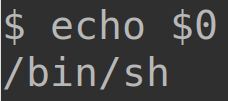
\includegraphics[width=0.5\textwidth,height=0.5\textheight,keepaspectratio]{images/bourne_shell.png}
	\end{center}
}

\frame{
	\frametitle{Bourne-Again Shell}
	\begin{itemize}
		\item Commonly located at \textbf{/bin/bash} and is the default shell for many Linux distributions
		\item The shell we will be looking at a lot today :)
	\end{itemize}
	
	
\includegraphics[width=\textwidth,height=0.9\textheight,keepaspectratio]{images/bash.jpg}
}

\frame{
	\frametitle{Quick note about other shells}
	There is so many other shells out there, but we will be focusing on BASH today. Personally I use oh my zsh at work and home, but it's all mostly a preference thing.
	
	\begin{center}
		
\includegraphics[width=0.5\textwidth,height=0.5\textheight,keepaspectratio]{images/OMZLogo_BnW.png}
	\end{center}
}

\frame{
	\frametitle{Other shells}
	\begin{itemize}
		\item zsh, fish are popular alternatives to bash
		\item Tcsh and Ksh are old favorites with strict POSIX compliance
		\item Ash, Dash lightweight so useful for embedded systems
		\item Powershell exists
	\end{itemize}
	\begin{center}
		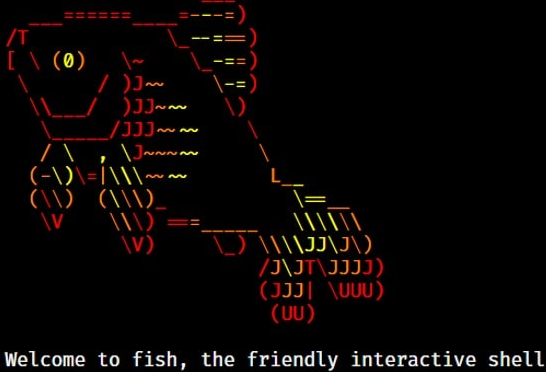
\includegraphics[width=0.5\textwidth,height=0.5\textheight,keepaspectratio]{images/fish.png}
	\end{center}
}



%%%%%%%%%% CONNECTING TO A REMOTE MACHINE

\section{Connecting to a Remote Machine}

\frame{
	\frametitle{SSH Client}
	If on Mac/Linux just open a terminal and use that \\
	
	If on Windows, use a SSH Client such as MobaXTerm/PuTTy
	
	\begin{columns}
		\column{0.5\linewidth}
		\centering
		
\includegraphics[width=0.5\textwidth,height=0.5\textheight,keepaspectratio]{images/MobaXTerm_Logo.jpg}
		\column{0.5\linewidth}
		\centering
		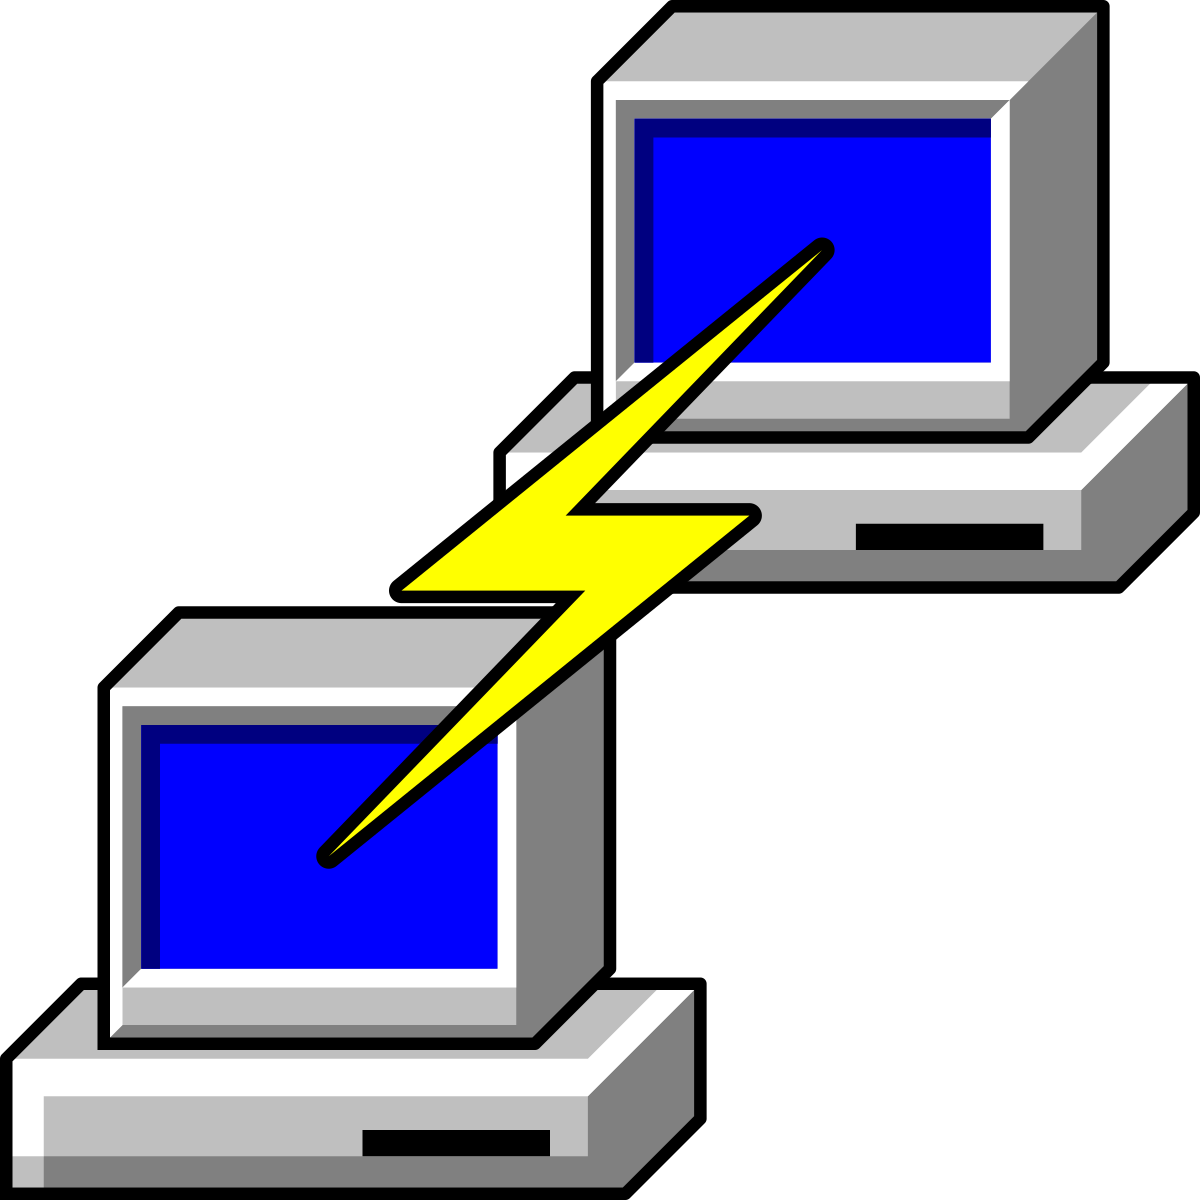
\includegraphics[width=0.5\textwidth,height=0.5\textheight,keepaspectratio]{images/PuTTy_icon.png}
	\end{columns}
}




\section{Playing around in Linux}


\frame{
	\frametitle{sudo}
	sudo is a \textbf{program} that enables regular users to run programs with security privileges of \textbf{another user}\\
	
	\begin{itemize}
		\item A good example is `sudo apt update` 
	\end{itemize}
	
	\textbf{Disclaimer}: If a random web page tells you to use sudo and you don't know what you're doing, don't do it.

	\begin{center}
		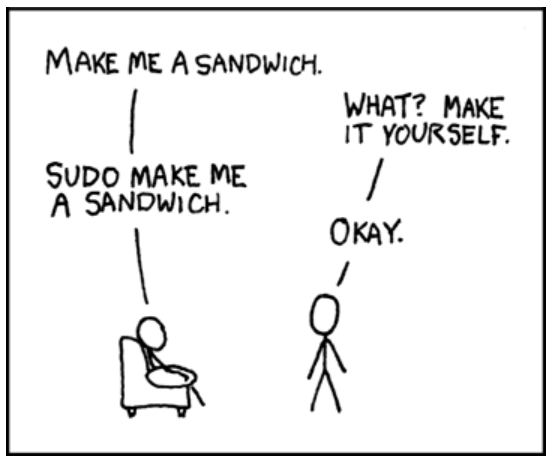
\includegraphics[width=0.5\textwidth,height=0.5\textheight,keepaspectratio]{images/xkcd_149.png}
	\end{center}

}


\frame{
	\frametitle{sudo - quick note}
	When using sudo you will be \textbf{prompted for a password}. There will be a grace period where when you use sudo again you won't have to input password. This can be dangerous if you, say, update your system, and then run some sketchy shell script that you aren't reading the contents of. If said shell script uses sudo for something then it will just get free access. \\
	
	This is why I always recommend running new shell scripts in a new shell (a container/vm is even better).
}


\frame{
	\frametitle{Basic Commands}
	\begin{itemize}
		\item `\textbf{pwd}` print working directory
		\item `\textbf{ls -l}` list contents of current directory with listing format
		\item `\textbf{mkdir test}` make a directory named "test"
		\item `\textbf{cd test}` change directory to the dir "test"
		\item `\textbf{touch file.txt}` create a file named "file.txt"
		\item `\textbf{file file.txt}` inspect what the file is
		\item `\textbf{rm file.txt}` remove the file
		\item `\textbf{echo "Hello!" $>$ file.txt}` redirect STDOUT to the file "file.txt"
	\end{itemize}
}

\frame{
	\frametitle{Shell Expansions}
	There are 8 different types of expansions: \textbf{brace expansion, tilde expansion, parameter expansion, arithmetic expansion, command substitution, word splitting, filename expansion}
	\begin{center}
		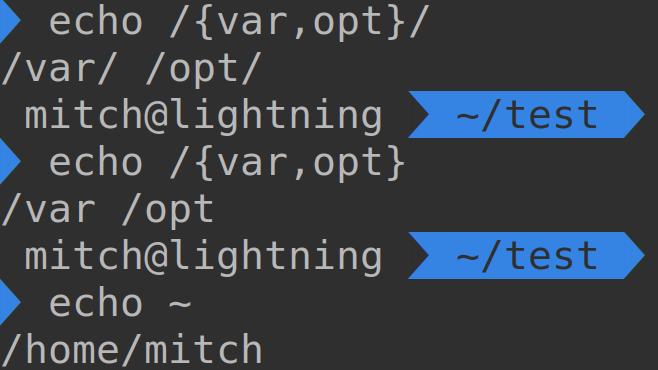
\includegraphics[width=0.7\textwidth,height=0.7\textheight,keepaspectratio]{images/shell_expansion1.png}
	\end{center}
}

\frame{
	\frametitle{Shell Expansions - filename and word splitting}
	We can expand filenames (*) and do word splitting [@] to find how many files there are ($\#$) in cwd
	\begin{center}
		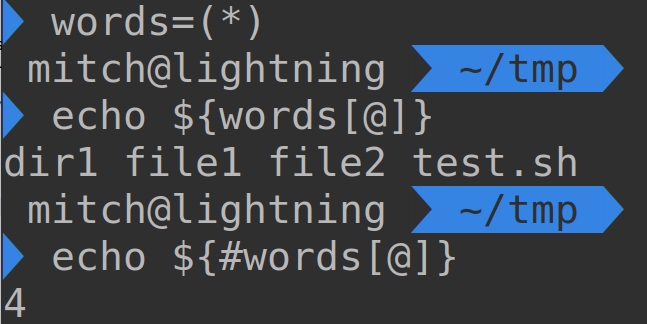
\includegraphics[width=0.7\textwidth,height=0.7\textheight,keepaspectratio]{images/shell_expansion_filename.png}
	\end{center}
}

\frame{
	\frametitle{Parameter Expansion}
	In our shell, we can set and use variables
	\begin{center}
		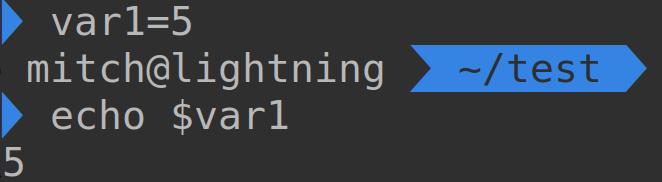
\includegraphics[width=\textwidth,height=\textheight,keepaspectratio]{images/var1.png}
	\end{center}
}

\frame{
	\frametitle{Parameter Expansion - sub strings}
	We can also print only specific parts of a string with the ":offset:length" operator
	\begin{center}
		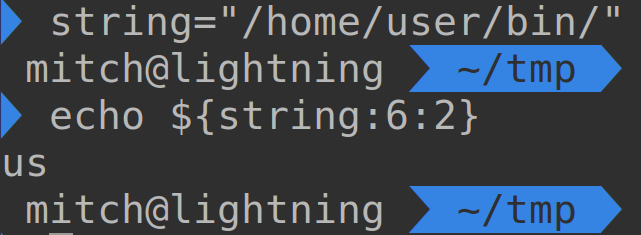
\includegraphics[width=\textwidth,height=\textheight,keepaspectratio]{images/parameter_expansion_sub.png}
	\end{center}
}

\frame{
	\frametitle{Math is fun}
	We can even do math with variables!
	\begin{center}
		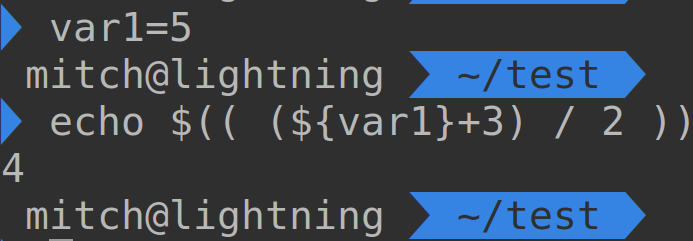
\includegraphics[width=\textwidth,height=\textheight,keepaspectratio]{images/mathisfun.png}
	\end{center}
}


\frame{
	\frametitle{Redirections}
	Basic Redirections
	\begin{itemize}
		\item echo "hello" $>$ file.txt \# overwrites file and writes hello
		\item date $>>$ file.txt \# appends output of date command to file
	\end{itemize}

	\textbf{File Descriptors}
	STDIN (0), STDOUT (1), STDERR (2)
	\begin{center}
		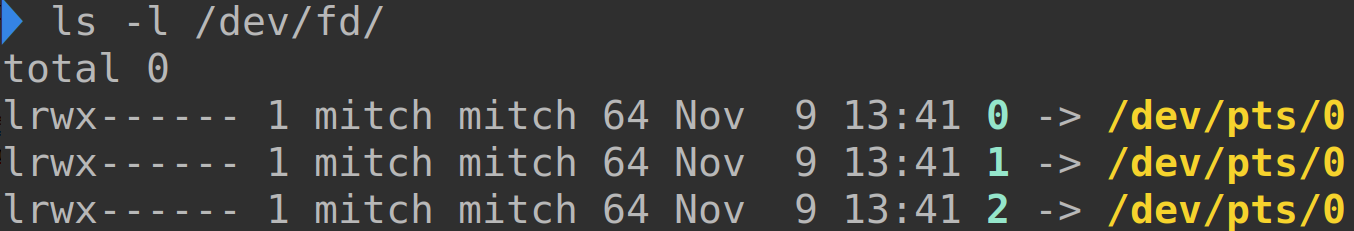
\includegraphics[width=\textwidth,height=\textheight,keepaspectratio]{images/ls_fd.png}
	\end{center}
}

\frame{
	\frametitle{Redirection - file descriptors}
	I can redirect only STDOUT to a file
	\begin{center}
		
\includegraphics[width=\textwidth,height=\textheight,keepaspectratio]{images/redirect_stdout.png}
	\end{center}
	I can redirect only STDERR to a file
	\begin{center}
		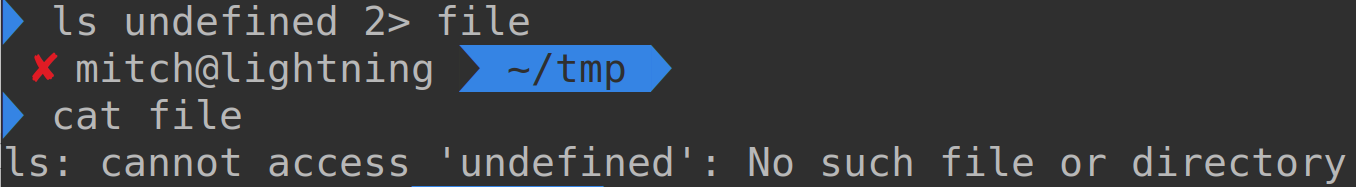
\includegraphics[width=\textwidth,height=\textheight,keepaspectratio]{images/redirect_stderr.png}
	\end{center}
}

\frame{
	\frametitle{Redirection - file descriptors 2}
	What if I want BOTH STDOUT and STDERR?
	\begin{center}
		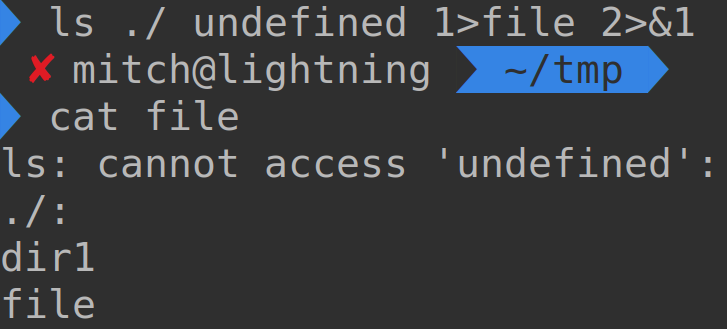
\includegraphics[width=\textwidth,height=\textheight,keepaspectratio]{images/redirect_both.png}
	\end{center}
}


\frame{
	\frametitle{Redirection - file descriptors 3}
	What if I just want to see STDOUT and not STDERR?
	\begin{center}
		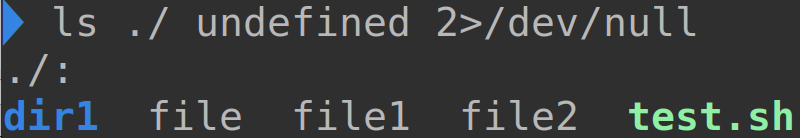
\includegraphics[width=\textwidth,height=\textheight,keepaspectratio]{images/redirect_reject_stdout.png}
	\end{center}
}

\frame{
	\frametitle{Redirection - Multiple Redirections}
	This is a fun example of something I do at work all the time
	\begin{center}
		
\includegraphics[width=\textwidth,height=\textheight,keepaspectratio]{images/32B_random.png}
	\end{center}
	Read left to right, we take the first 32 Bytes of /dev/random and redirect that to a file
}


\frame{
	\frametitle{Pipes}
	Pipes are similar to redirection commands, except it works to connect the STDOUT of one comment to the STDIN of another command
	\begin{center}
		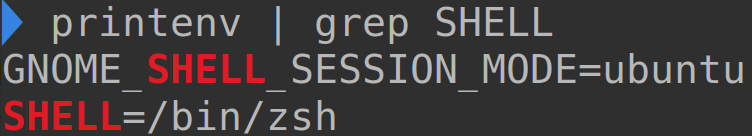
\includegraphics[width=\textwidth,height=\textheight,keepaspectratio]{images/printenv_grep.png}
	\end{center}
	In this case, printenv writes to STDOUT, and that is redirected to STDIN of grep
}

\frame{
	\frametitle{Pipes - real life example}
	This is a string of commands that will kill all firefox instances
	\begin{center}
		
\includegraphics[width=\textwidth,height=\textheight,keepaspectratio]{images/kill_firefox.png}
	\end{center}
}


\frame{
	\frametitle{Exit Status}
	All commands have an exit status
	\begin{center}
		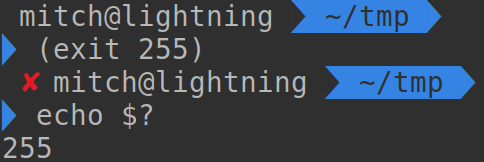
\includegraphics[width=0.75\textwidth,height=0.75\textheight,keepaspectratio]{images/sp_rc.png}
	\end{center}
	These are convenient ways for scripts to know how the last command went
}

\frame{
	\frametitle{\&\& and $||$}
	\&\& (AND) will do the second command only if the first command is successful\\
	$||$ (OR) will do the second command if the first command fails
	
	\begin{center}
		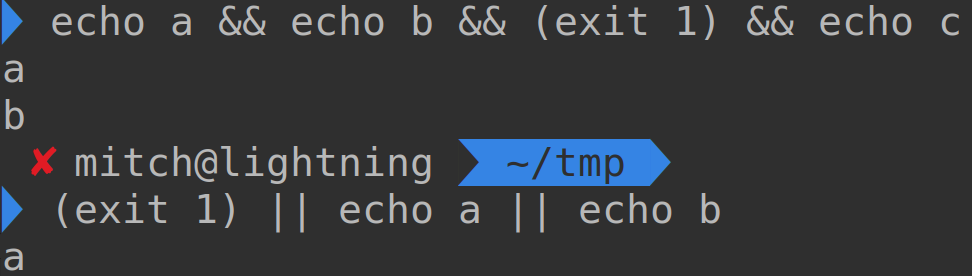
\includegraphics[width=\textwidth,height=\textheight,keepaspectratio]{images/exit_chaining.png}
	\end{center}
}


\frame{
	\frametitle{Conditional Expressions}
	\begin{center}
		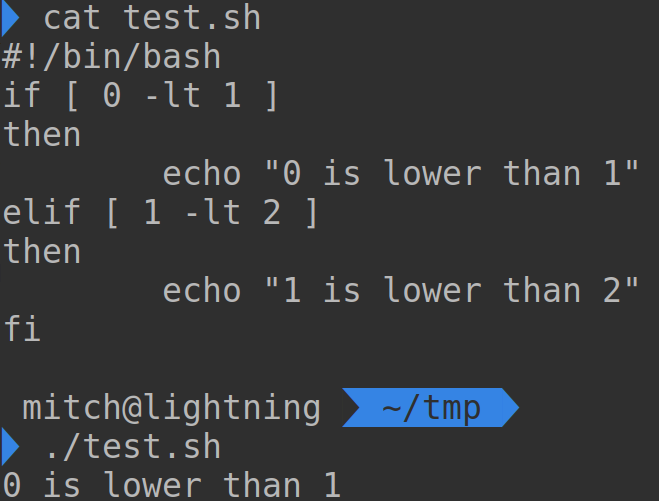
\includegraphics[width=0.8\textwidth,height=0.8\textheight,keepaspectratio]{images/conditional_construct.png}
	\end{center}
}

\frame{
	\frametitle{Conditional Expressions 2}
	You bet we got case statements too!
	\begin{center}
		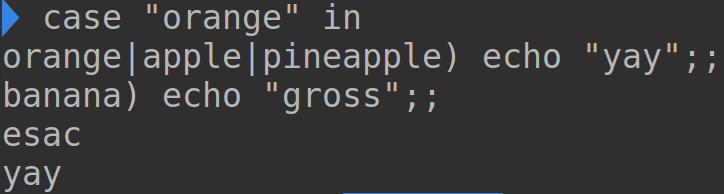
\includegraphics[width=0.8\textwidth,height=0.8\textheight,keepaspectratio]{images/case_statement.png}
	\end{center}
}

\frame{
	\frametitle{Conditional Expressions 3}
	We can also check that a file exists with -a
	\begin{center}
		\includegraphics[width=\textwidth,height=\textheight,keepaspectratio]{images/test_file_existence.png}
	\end{center}
}



\frame{
	\frametitle{Loops}
	We have just basic for loops
	\begin{center}
		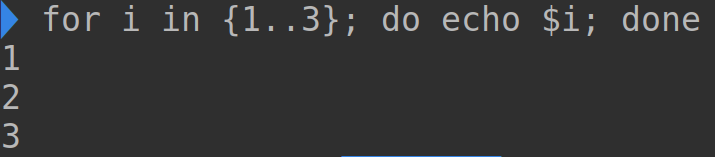
\includegraphics[width=\textwidth,height=\textheight,keepaspectratio]{images/for_loop.png}
	\end{center}
}

\frame{
	\frametitle{Loops}
	We can mix file expansion to do a certain operation with multiple files
	\begin{center}
		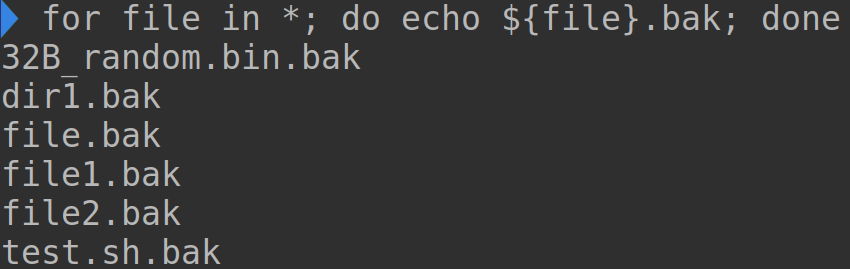
\includegraphics[width=\textwidth,height=\textheight,keepaspectratio]{images/for_file_expansion.png}
	\end{center}
}


\section{Writing Our own Shell Scripts}

\frame{
	\frametitle{Shebang}
	A sheband (haSH BANG) is at the top of script files to be ran with a certain interpreter
	\begin{center}
		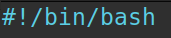
\includegraphics[width=0.5\textwidth,height=0.5\textheight,keepaspectratio]{images/shebang.png}
	\end{center}
	In the above example, \textbf{/bin/bash} is being used as the interpreter
}

\frame{
	\frametitle{Functions}
	Functions are a way for you to define a set of commands to reuse
	\begin{center}
		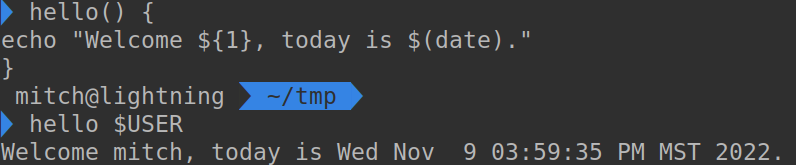
\includegraphics[width=\textwidth,height=\textheight,keepaspectratio]{images/function_hello.png}
	\end{center}
}


\frame{
	\frametitle{Special Parameters}
	The first special parameter is positional arguments, this is how you can receive arguments from the commandline
	\begin{center}
		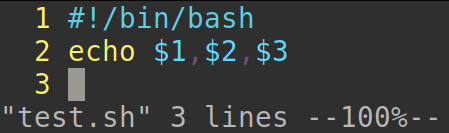
\includegraphics[width=0.5\textwidth,height=0.5\textheight,keepaspectratio]{images/special_params_sc.png}
		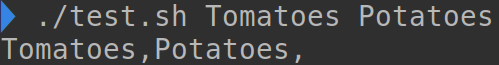
\includegraphics[width=0.5\textwidth,height=0.5\textheight,keepaspectratio]{images/special_params.png}
	\end{center}
	
	In the above image I give the positional arguments Tomatoes (\$1) and Potatoes (\$2) and nothing to \$3\\
	
	What do you think \$0 will print out?
	
}

\frame{
	\frametitle{Special Parameters - Expand}
	What if you want each positional argument printed as a word?
	\begin{center}
		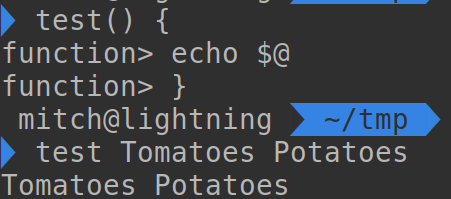
\includegraphics[width=0.8\textwidth,height=0.8\textheight,keepaspectratio]{images/sp_expand.png}
	\end{center}
	\$@ got you covered
}

\frame{
	\frametitle{Special Parameters - IFS}
	IFS stands for Internal Field Separator
	
	\begin{center}
		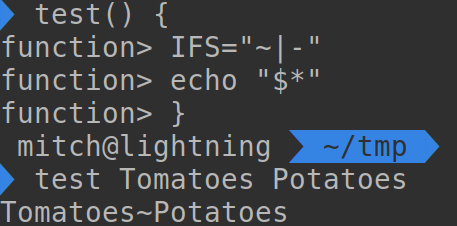
\includegraphics[width=0.8\textwidth,height=0.8\textheight,keepaspectratio]{images/sp_IFS.png}
	\end{center}	
}


\frame{
	\frametitle{Special Parameters - num arguments, exit status}
	You can also get the number of arguments
	\begin{center}
		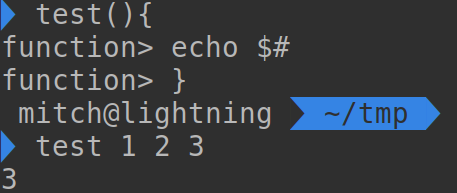
\includegraphics[width=0.5\textwidth,height=0.5\textheight,keepaspectratio]{images/sp_num_arguments.png}
	\end{center}
	And you can also print the return code from the last ran command
	\begin{center}
		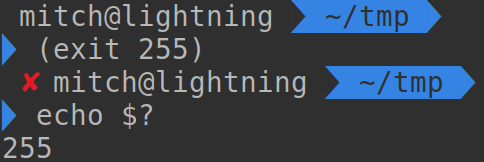
\includegraphics[width=0.5\textwidth,height=0.5\textheight,keepaspectratio]{images/sp_rc.png}
	\end{center}	
}

\frame{
	\frametitle{Special Parameters - Recap}
	Recap of special parameters
	\begin{itemize}
		\item \$1, \$2, \$3 are the value of positional arguments
		\item \$0 expands the name of the bash script
		\item \$@ turns all positional arguments into a single word
		\item echo "\$*" expands positional arguments by IFS
		\item \$\# expands number of positional arguments
		\item \$? Exit status from recent command
	\end{itemize}
}

\frame{
	\frametitle{lstree}
	\begin{center}
	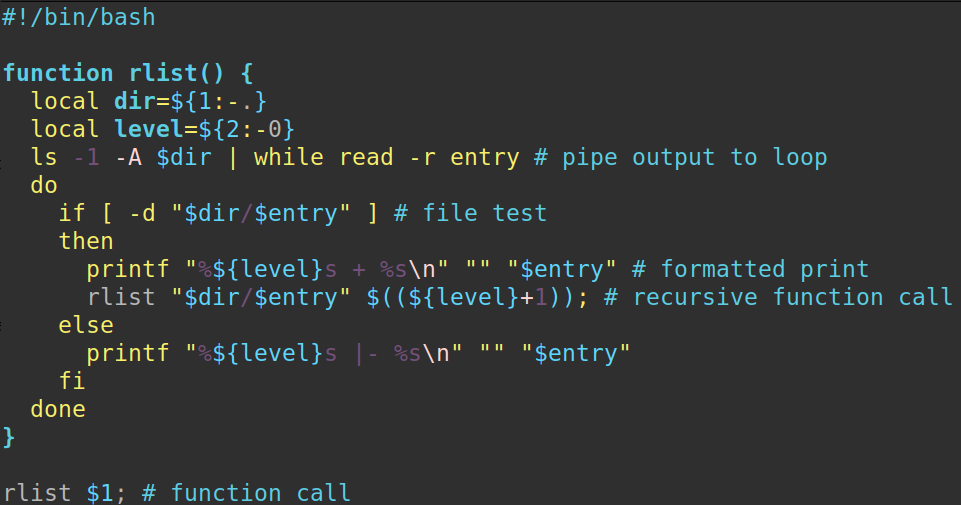
\includegraphics[width=\textwidth,height=\textheight,keepaspectratio]{images/lstree.png}
\end{center}	
}

\frame{
	\frametitle{Thanks}
	Thanks Peter Andreas Möller, as I stole your lstree source code	and some lesson structure.
}
\end{document}
